% !TEX TS-program = lualatexmk
% !TEX parameter =  --shell-escape
\documentclass[benediction_assumption_la_en.tex]{subfiles}

\ifcsname preamble@file\endcsname
  \setcounter{page}{\getpagerefnumber{M-benediction_assumption_la_en_after_benediction}}
\fi

\begin{document}

\chapter*{AFTER BENEDICTION.}
\addcontentsline{toc}{chapter}{After Benediction}
\header{after benediction.}

\label{divine_praises}
\bigtitle{The Divine Praises.}

\textes{laudes_divinae_en}

\rubrique{These are sung alternating between the cantors and the whole congregation. All sing \normaltext{Fiat, Fiat} at the end.}

\rubrique{Tone of the abbey of Maredsous, Belgium.}

%\gscore[]{}{laudes_divinae_no_breaks}
\idxscore{laudes_divinae_no_breaks}{}{Va}{Laudes Divinæ, tone of Maredsous Abbey}

\bigtitle{Reposition.}

\rubrique{As the priest or deacon begins to repose the Blessed Sacrament, one of the following chants is sung immediately.}

\smalltitle{On Major Feasts.}

\rubrique{Adapted from chant used by the French royal chapel and at Notre-Dame de Paris.}

\rubrique{
\begin{enpars}
 The cantors sing the odd verses, all others evens. On the greatest occasions, the even verses may be sung in fauxbourdon or supplied by the organ.\end{enpars}}

%\gscore[]{6.}{ps_laudate_dominum_ton_royal}
\idxscore{ps_laudate_dominum_ton_royal}[\textit{Ton roy.}]{6.}{Ps}{Laudate Dominum, ton royal}

\textes{ps_116_en}
\newpage
\smalltitle{On Sundays \textit{per annum} and until Ash Wednesday.}

\rubrique{The cantors intone until the quarter bar and intone each verse until the asterisk.}

\rubrique{Melody adapted ca. 1895, probably by Dom Joseph Pothier, o.s.b.}

%\gscore[]{5.}{va_adoremus_in_aeternum_solesmes_1961}
\idxscore{va_adoremus_in_aeternum_solesmes_1961}{5.}{Va}{Adoremus in æternum, in mode 5}
\textes{Adoremus_in_aeternum_en}

\smalltitle{In Advent and Lent.}

%\gscore[]{6.}{Adoremus_westminster_mode_6}
\idxscore{Adoremus_westminster_mode_6}{6.}{Va}{Adoremus, Westminster tone in mode 6}

%\textes{Adoremus_in_aeternum_en}

\smalltitle{In Paschal Time.}

\rubrique{The cantors sing the odd verses, all others evens.}

\rubrique{Psalm tone for psalms without an antiphon in Paschal Time from the \normaltext{Antiphonale Romanum.}}

%\gscore[]{}{ps_116_tp}
\idxscore{ps_116_tp}{}{Ps}{Laudate Dominum, tone in Paschal Time}
%\textes{ps_116_en}
%\newpage
\label{holy_god_we_praise_thy_name}  \phantomsection
\smalltitle{On Weekdays \textit{ per annum.}}

\index[Hy]{Holy God, We Praise Thy Name, GROSSER GOTT}
{\centering{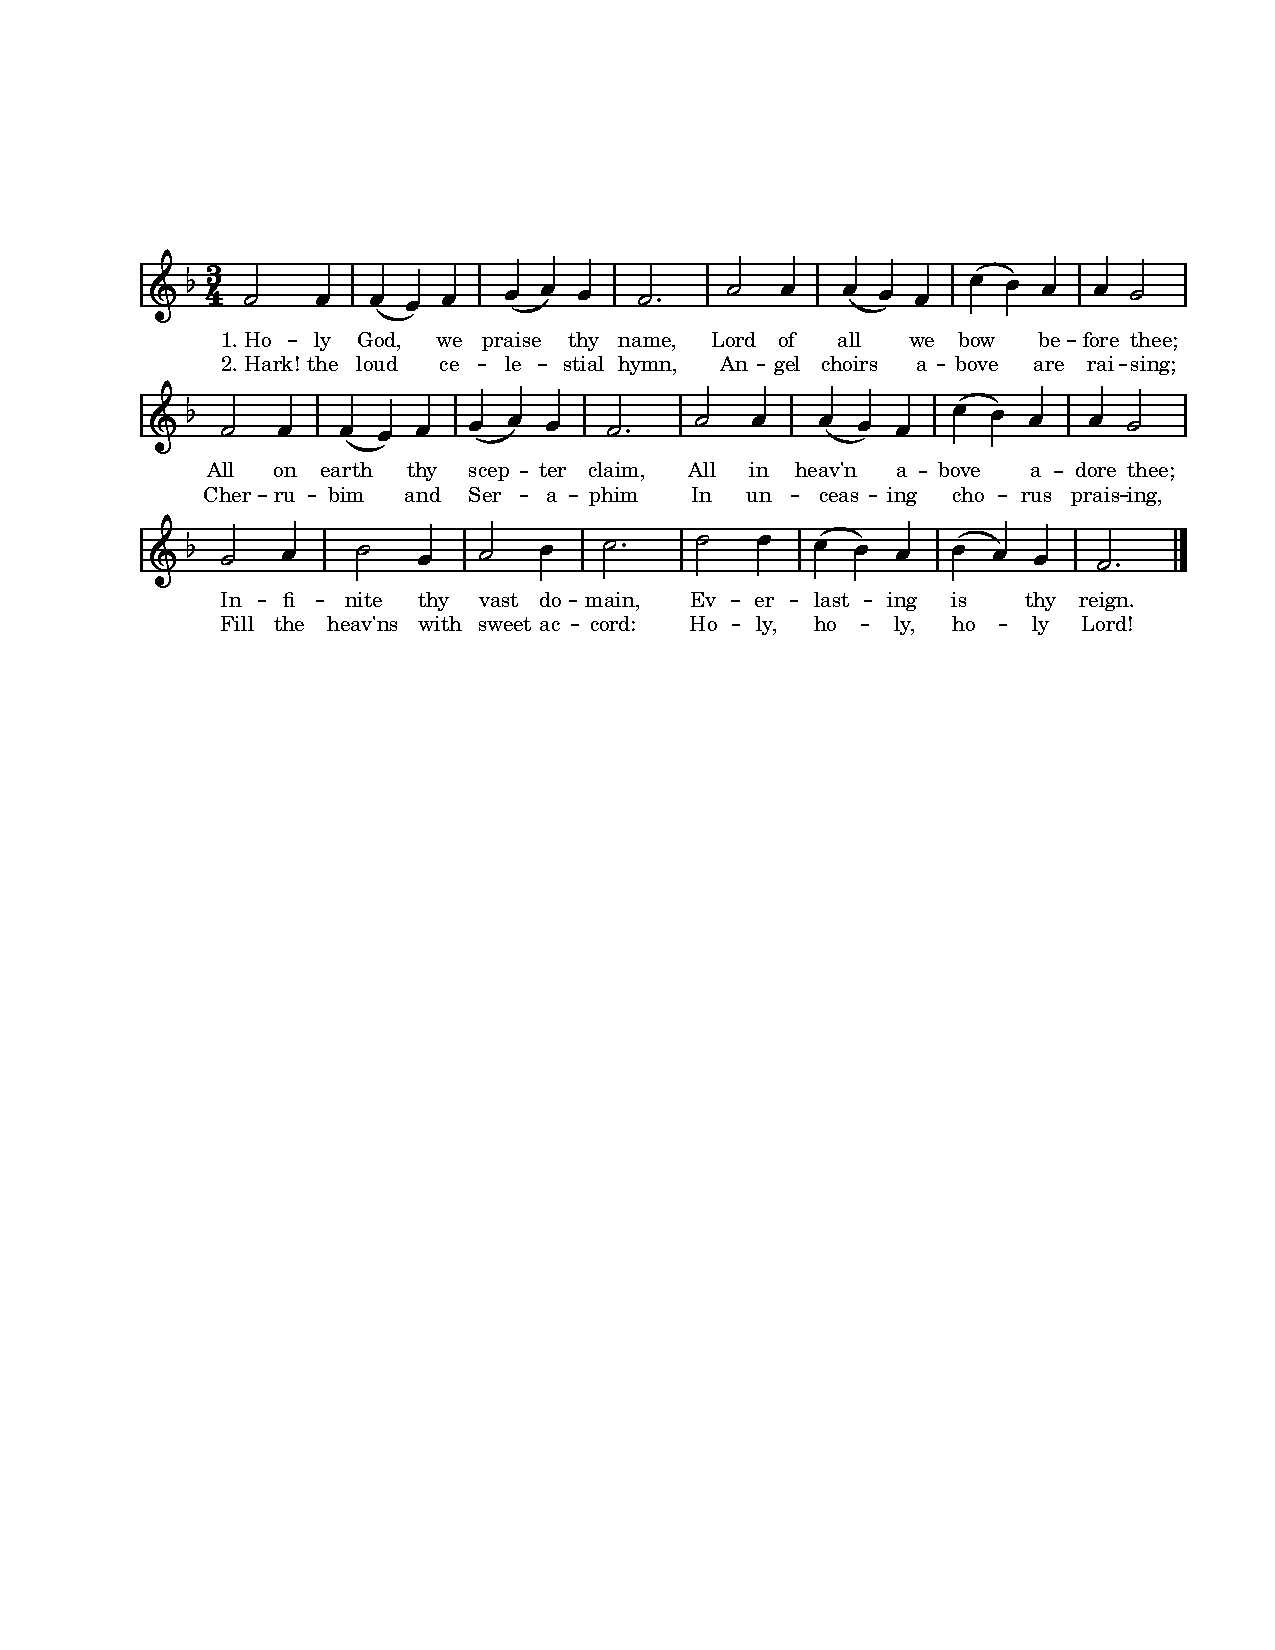
\includegraphics[scale=0.75,keepaspectratio]{holy_god_we_praise_thy_name_melody_cropped}\par}}

\newpage

\rubrique{Or}

\vspace{0.25\baselineskip}

%{\centering{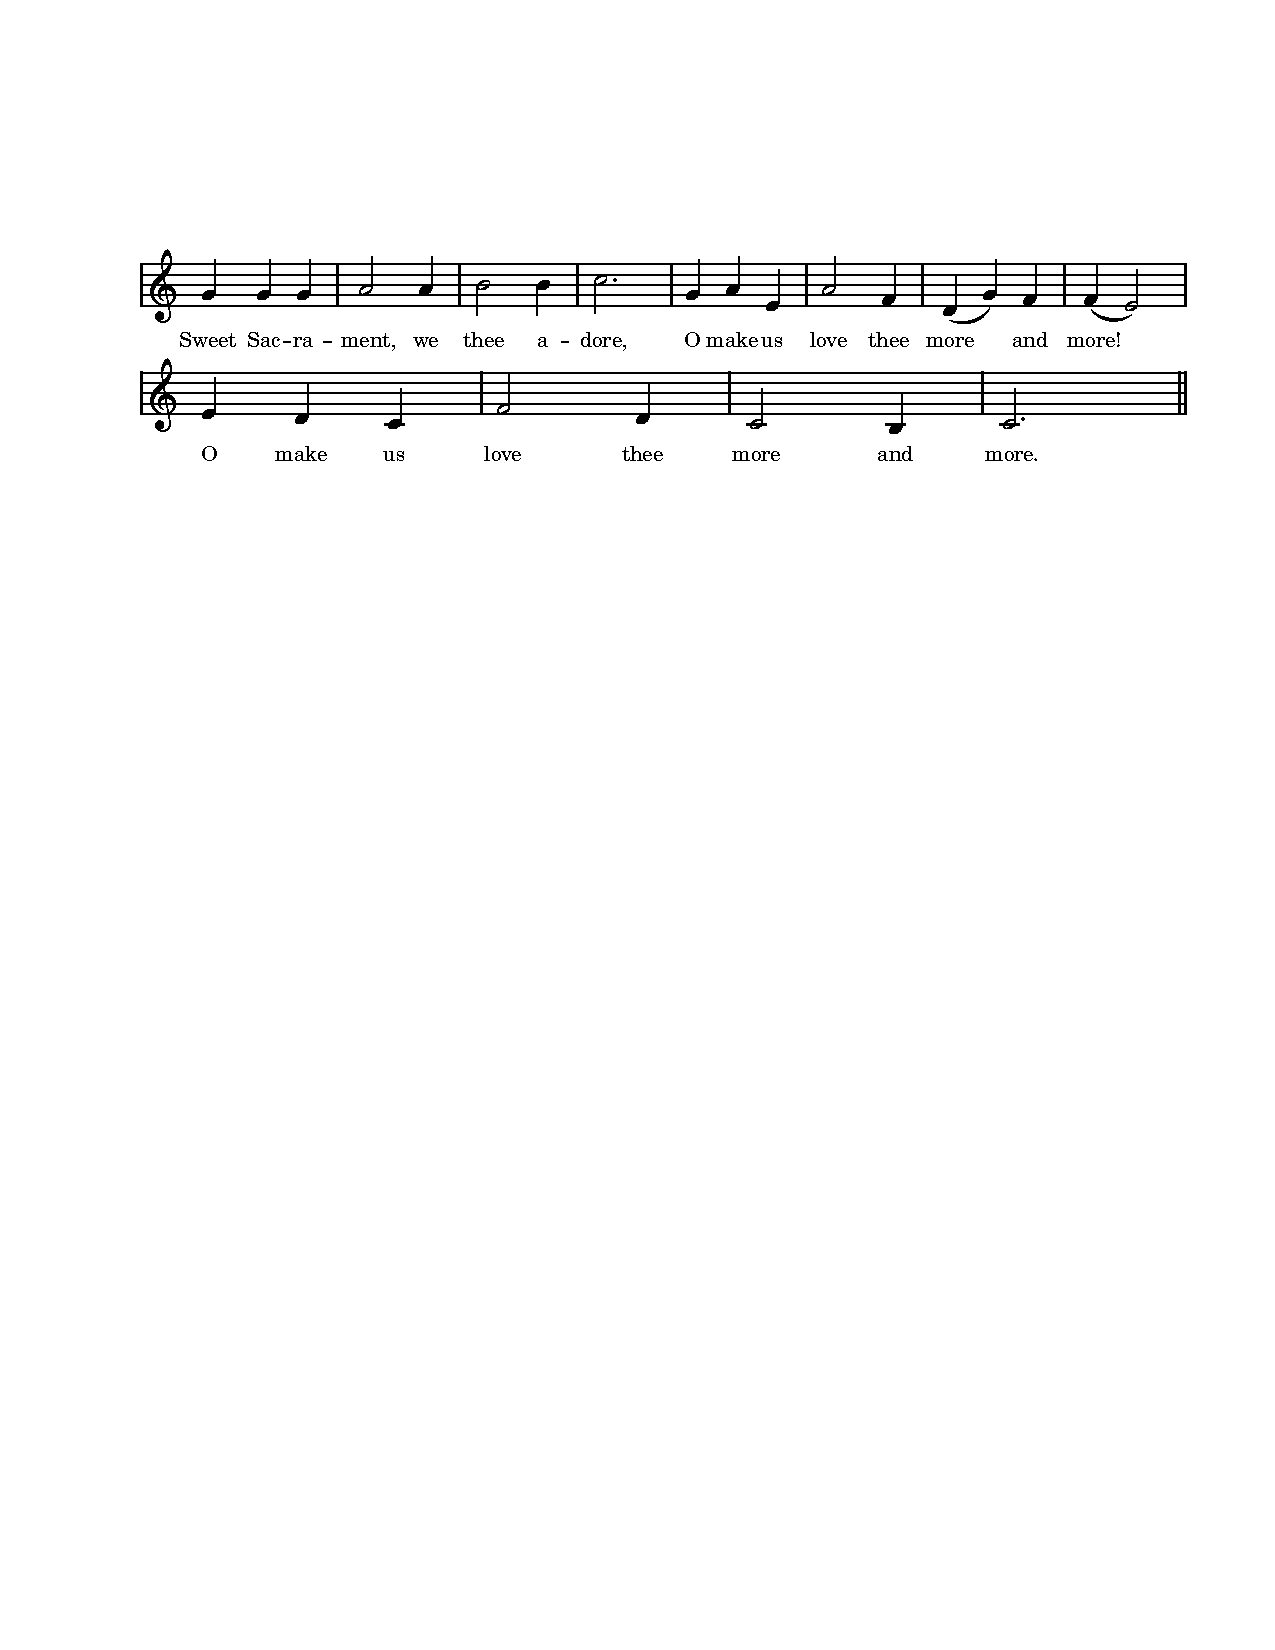
\includegraphics[width=100mm,height=500mm,keepaspectratio]{sweet_sacrament_melody}\par}}
{\centering{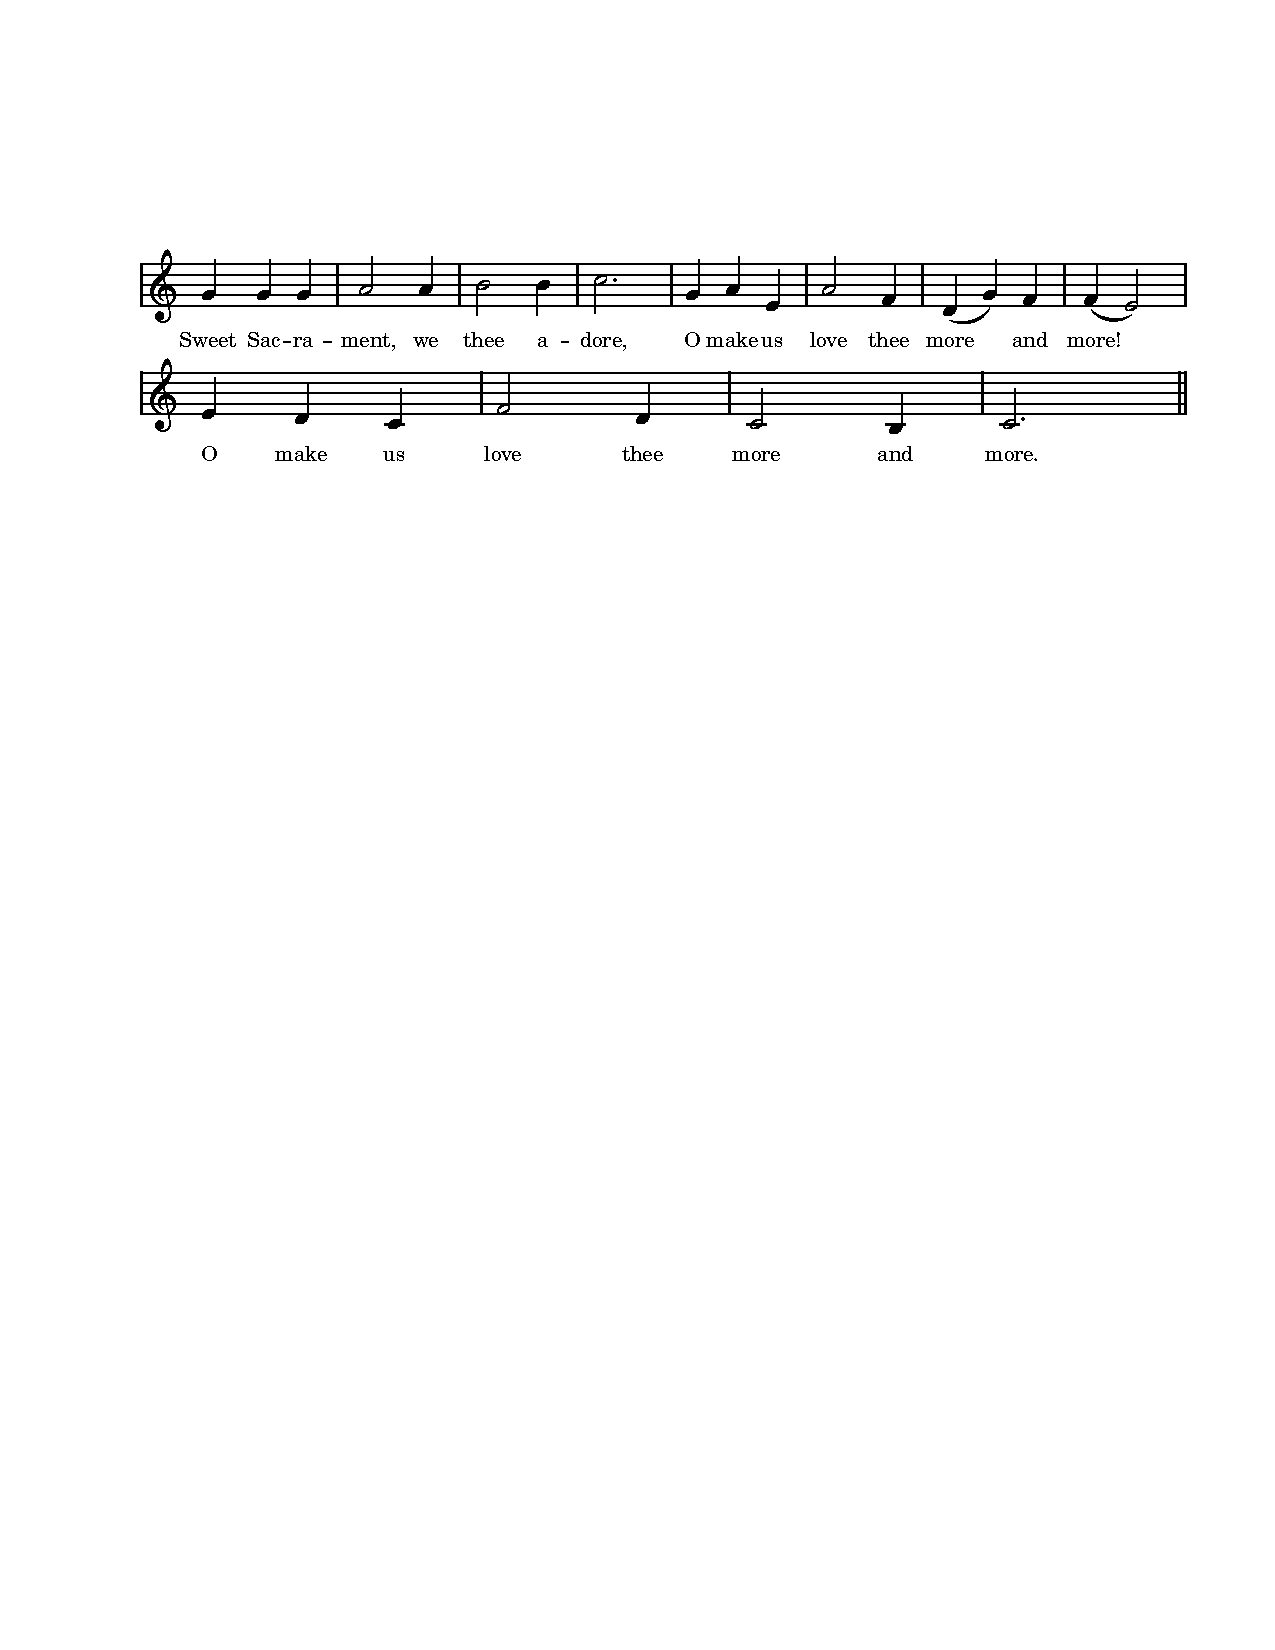
\includegraphics[scale=0.75,keepaspectratio]{sweet_sacrament_melody}\par}}

\smalltitle{In the month of June and on First Friday, after the distribution of communion.} \label{cor_jesu} \phantomsection

\rubrique{
\begin{enpars}The cantors intone until the half bar, then all sing the rest of the antiphon and the repetitions.\end{enpars}}

\rubrique{Melody adapted, probably by Dom Joseph Pothier, o.s.b.}

%\gscore[]{1.}{va_cor_jesu_solesmes}
\idxscore{va_cor_jesu_solesmes}[]{1.}{Va}{Cor Jesus sacratissimum, mode 1}
\textes{Cor_Jesu_en}

\end{document}